
\newpage
\section*{\emph{If---}}
\paragraph{By Rudyard Kippling}~
\begin{verse}
	If you can keep your head when all about you\\
	\hspace{0.5em} Are losing theirs and blaming it on you,\\
	If you can trust yourself when all men doubt you,\\
	\hspace{0.5em} But make allowance for their doubting too;\\
	If you can wait and not be tired by waiting,\\
	\hspace{0.5em} Or being lied about, don’t deal in lies,\\
	Or being hated, don’t give way to hating,\\
	\hspace{0.5em} And yet don’t look too good, nor talk too wise:

	If you can dream—and not make dreams your master;\\
	\hspace{0.5em} If you can think—and not make thoughts your aim;\\
	If you can meet with Triumph and Disaster\\
	\hspace{0.5em} And treat those two impostors just the same;\\
	If you can bear to hear the truth you’ve spoken\\
	\hspace{0.5em} Twisted by knaves to make a trap for fools,\\
	Or watch the things you gave your life to, broken,\\
	\hspace{0.5em} And stoop and build ’em up with worn-out tools:

	If you can make one heap of all your winnings\\
	\hspace{0.5em} And risk it on one turn of pitch-and-toss,\\
	And lose, and start again at your beginnings\\
	\hspace{0.5em} And never breathe a word about your loss;\\
	If you can force your heart and nerve and sinew\\
	\hspace{0.5em} To serve your turn long after they are gone,\\
	And so hold on when there is nothing in you\\
	\hspace{0.5em} Except the Will which says to them: ‘Hold on!’

	If you can talk with crowds and keep your virtue,\\
	\hspace{0.5em} Or walk with Kings—nor lose the common touch,\\
	If neither foes nor loving friends can hurt you,\\
	\hspace{0.5em} If all men count with you, but none too much;\\
	If you can fill the unforgiving minute\\
	\hspace{0.5em} With sixty seconds’ worth of distance run,\\
	Yours is the Earth and everything that’s in it,\\
	\hspace{0.5em} And—which is more—you’ll be a Man, my son!
\end{verse}



\newpage
\section*{\emph{Sonnet 18: Shall I compare thee to a summer’s day?}}
\paragraph{By William Shakespeare}~
\begin{verse}
	Shall I compare thee to a summer’s day?\\
	Thou art more lovely and more temperate:\\
	Rough winds do shake the darling buds of May,\\
	And summer’s lease hath all too short a date;\\
	Sometime too hot the eye of heaven shines,\\
	And often is his gold complexion dimm'd;\\
	And every fair from fair sometime declines,\\
	By chance or nature’s changing course untrimm'd;\\
	But thy eternal summer shall not fade,\\
	Nor lose possession of that fair thou ow’st;\\
	Nor shall death brag thou wander’st in his shade,\\
	When in eternal lines to time thou grow’st:\\
	\hspace{0.5em} So long as men can breathe or eyes can see,\\
	\hspace{0.5em} So long lives this, and this gives life to thee.
\end{verse}

\newpage
\newgeometry{vmargin=1.2in, hmargin=1.2in}
\section*{\emph{The Cremation of Sam McGee}}
\paragraph{By Robert W. Service}~
\begin{verse}
	{\itshape
		There are strange things done in the midnight sun\\
		\hspace{0.5em} By the men who moil for gold;\\
		The Arctic trails have their secret tales\\
		\hspace{0.5em} That would make your blood run cold;\\
		The Northern Lights have seen queer sights,\\
		\hspace{0.5em} But the queerest they ever did see\\
		Was that night on the marge of Lake Lebarge\\
		\hspace{0.5em} I cremated Sam McGee.
	}

	Now Sam McGee was from Tennessee, where the cotton blooms and blows.\\
	Why he left his home in the South to roam 'round the Pole, God only knows.\\
	He was always cold, but the land of gold seemed to hold him like a spell;\\
	Though he'd often say in his homely way that “he'd sooner live in hell.”

	On a Christmas Day we were mushing our way over the Dawson trail.\\
	Talk of your cold! through the parka's fold it stabbed like a driven nail.\\
	If our eyes we'd close, then the lashes froze till sometimes we couldn't see;\\
	It wasn't much fun, but the only one to whimper was Sam McGee.

	And that very night, as we lay packed tight in our robes beneath the snow,\\
	And the dogs were fed, and the stars o'erhead were dancing heel and toe,\\
	He turned to me, and “Cap,” says he, “I'll cash in this trip, I guess;\\
	And if I do, I'm asking that you won't refuse my last request.”

	Well, he seemed so low that I couldn't say no; then he says with a sort of moan:\\
	“It's the cursèd cold, and it's got right hold till I'm chilled clean through to the bone.\\
	Yet 'tain't being dead—it's my awful dread of the icy grave that pains;\\
	So I want you to swear that, foul or fair, you'll cremate my last remains.”

	A pal's last need is a thing to heed, so I swore I would not fail;\\
	And we started on at the streak of dawn; but God! he looked ghastly pale.\\
	He crouched on the sleigh, and he raved all day of his home in Tennessee;\\
	And before nightfall a corpse was all that was left of Sam McGee.

	There wasn't a breath in that land of death, and I hurried, horror-driven,\\
	With a corpse half hid that I couldn't get rid, because of a promise given;\\
	It was lashed to the sleigh, and it seemed to say: “You may tax your brawn and brains,\\
	But you promised true, and it's up to you to cremate those last remains.”

	Now a promise made is a debt unpaid, and the trail has its own stern code.\\
	In the days to come, though my lips were dumb, in my heart how I cursed that load.\\
	In the long, long night, by the lone firelight, while the huskies, round in a ring,\\
	Howled out their woes to the homeless snows— O God! how I loathed the thing.

	And every day that quiet clay seemed to heavy and heavier grow;\\
	And on I went, though the dogs were spent and the grub was getting low;\\
	The trail was bad, and I felt half mad, but I swore I would not give in;\\
	And I'd often sing to the hateful thing, and it hearkened with a grin.

	Till I came to the marge of Lake Lebarge, and a derelict there lay;\\
	It was jammed in the ice, but I saw in a trice it was called the “Alice May.”\\
	And I looked at it, and I thought a bit, and I looked at my frozen chum;\\
	Then “Here,” said I, with a sudden cry, “is my cre-ma-tor-eum.”

	Some planks I tore from the cabin floor, and I lit the boiler fire;\\
	Some coal I found that was lying around, and I heaped the fuel higher;\\
	The flames just soared, and the furnace roared—such a blaze you seldom see;\\
	And I burrowed a hole in the glowing coal, and I stuffed in Sam McGee.

	Then I made a hike, for I didn't like to hear him sizzle so;\\
	And the heavens scowled, and the huskies howled, and the wind began to blow.\\
	It was icy cold, but the hot sweat rolled down my cheeks, and I don't know why;\\
	And the greasy smoke in an inky cloak went streaking down the sky.

	I do not know how long in the snow I wrestled with grisly fear;\\
	But the stars came out and they danced about ere again I ventured near;\\
	I was sick with dread, but I bravely said: “I'll just take a peep inside.\\
	I guess he's cooked, and it's time I looked”; ... then the door I opened wide.

	And there sat Sam, looking cool and calm, in the heart of the furnace roar;\\
	And he wore a smile you could see a mile, and he said: “Please close that door.\\
	It's fine in here, but I greatly fear you'll let in the cold and storm—\\
	Since I left Plumtree, down in Tennessee, it's the first time I've been warm.”

	{\itshape
	There are strange things done in the midnight sun\\
	\hspace{0.5em} By the men who moil for gold;\\
	The Arctic trails have their secret tales\\
	\hspace{0.5em} That would make your blood run cold;\\
	The Northern Lights have seen queer sights,\\
	\hspace{0.5em} But the queerest they ever did see\\
	Was that night on the marge of Lake Lebarge\\
	\hspace{0.5em} I cremated Sam McGee.
	}
\end{verse}

\newpage
\newgeometry{margin=1.25in}
\section*{\emph{A Litany for Survival}}
\paragraph{By Audre Lorde}~

\vspace{1em}\noindent
\begin{minipage}[t]{0.56\linewidth}
	For those of us who live at the shoreline\\
	standing upon the constant edges of decision\\
	crucial and alone\\
	for those of us who cannot indulge\\
	the passing dreams of choice\\
	who love in doorways coming and going\\
	in the hours between dawns\\
	looking inward and outward\\
	at once before and after\\
	seeking a now that can breed\\
	futures\\
	like bread in our children’s mouths\\
	so their dreams will not reflect\\
	the death of ours;

	For those of us\\
	who were imprinted with fear\\
	like a faint line in the center of our foreheads\\
	learning to be afraid with our mother’s milk\\
	for by this weapon\\
	this illusion of some safety to be found\\
	the heavy-footed hoped to silence us\\
	For all of us\\
	this instant and this triumph\\
	We were never meant to survive.
\end{minipage}
\begin{minipage}[t]{0.45\linewidth}
	And when the sun rises we are afraid\\
	it might not remain\\
	when the sun sets we are afraid\\
	it might not rise in the morning\\
	when our stomachs are full we are afraid\\
	of indigestion\\
	when our stomachs are empty we are afraid\\
	we may never eat again\\
	when we are loved we are afraid\\
	love will vanish\\
	when we are alone we are afraid\\
	love will never return\\
	and when we speak we are afraid\\
	our words will not be heard\\
	nor welcomed\\
	but when we are silent\\
	we are still afraid

	So it is better to speak\\
	remembering\\
	we were never meant to survive.
\end{minipage}

\newpage
\section*{\emph{O Captain! My Captain!}}
\paragraph{By Walt Whitman}~
\begin{verse}
	O Captain! my Captain! our fearful trip is done,\\
	The ship has weather’d every rack, the prize we sought is won,\\
	The port is near, the bells I hear, the people all exulting,\\
	While follow eyes the steady keel, the vessel grim and daring;\\
	\hspace{7em} But O heart! heart! heart!\\
	\hspace{8em} O the bleeding drops of red,\\
	\hspace{9em} Where on the deck my Captain lies,\\
	\hspace{10em} Fallen cold and dead.

	O Captain! my Captain! rise up and hear the bells;\\
	Rise up—for you the flag is flung—for you the bugle trills,\\
	For you bouquets and ribbon’d wreaths—for you the shores a-crowding,\\
	For you they call, the swaying mass, their eager faces turning;\\
	\hspace{7em} Here Captain! dear father!\\
	\hspace{8em} This arm beneath your head!\\
	\hspace{9em} It is some dream that on the deck,\\
	\hspace{10em} You’ve fallen cold and dead.

	My Captain does not answer, his lips are pale and still,\\
	My father does not feel my arm, he has no pulse nor will,\\
	The ship is anchor’d safe and sound, its voyage closed and done,\\
	From fearful trip the victor ship comes in with object won;\\
	\hspace{7em} Exult O shores, and ring O bells!\\
	\hspace{8em} But I with mournful tread,\\
	\hspace{9em} Walk the deck my Captain lies,\\
	\hspace{10em} Fallen cold and dead.
\end{verse}

\newpage
\section*{\emph{Элегия (Elegy)}}
\paragraph{By Александр Сергеевич Пушкин (Alexander Sergeyevich Pushkin)}~
\begin{verse}
	Безумных лет угасшее веселье\\
	Мне тяжело, как смутное похмелье.\\
	Но, как вино — печаль минувших дней\\
	В моей душе чем старе, тем сильней.\\
	Мой путь уныл. Сулит мне труд и горе\\
	Грядущего волнуемое море.

	Но не хочу, о други, умирать;\\
	Я жить хочу, чтоб мыслить и страдать;\\
	И ведаю, мне будут наслажденья\\
	Меж горестей, забот и треволненья:\\
	Порой опять гармонией упьюсь,\\
	Над вымыслом слезами обольюсь,\\
	И может быть — на мой закат печальный\\
	Блеснет любовь улыбкою прощальной.
\end{verse}

\vspace{2em}
\begin{verse}
	The vanished joy of my crazy years\\
	Is as heavy as gloomy hang-over.\\
	But, like wine, the sorrow of past days\\
	Is stronger with time.\\
	My path is sad. The waving sea of the future\\
	Promises me only toil and sorrow.

	But, O my friends, I do not wish to die,\\
	I want to live – to think and suffer.\\
	I know, I’ll have some pleasures\\
	Among woes, cares and troubles.\\
	Sometimes I’ll be drunk with harmony again,\\
	Or will weep over my visions,\\
	And it’s possible, at my sorrowful decline,\\
	Love will flash with a parting smile
\end{verse}

\newpage
\section*{\emph{{\fontspec{Malgun Gothic}귀천} (Back to Heaven)}}
\paragraph{By {\fontspec{Malgun Gothic}천상병} (Cheon Sang-byeong)}~

{\fontspec{Malgun Gothic}
\begin{verse}
	나 하늘로 돌아가리라\\
	새벽빛 와 닿으면 스러지는\\
	이슬 더불어 손에 손을 잡고,

	나 하늘로 돌아가리라.\\
	노을빛 함께 단둘이서\\
	기슭에서 놀다가 구름 손짓하며는,

	나 하늘로 돌아가리라.\\
	아름다운 이 세상 소풍 끝내는 날,\\
	가서, 아름다웠더라고 말하리라...
\end{verse}
}

\vspace{2em}
\begin{verse}
	I'll go back to heaven again\\
	hand in hand with the dew\\
	that melts at the touch of the dawning day,

	I'll go back to heaven again.\\
	After playing on the slopes with the dusk,\\
	when the clouds beckon,

	I'll go back to heaven again.\\
	On the last day of my outing to this beautiful world,\\
	I'll go back and say: it was beautiful...
\end{verse}

\newpage
\section*{\emph{My Voice}}
\paragraph{By Rafael Campo}~
\begin{verse}
	To cure myself of wanting Cuban songs,\\
	I wrote a Cuban song about the need\\
	For people to suppress their fantasies,\\
	Especially unhealthy ones. The song\\
	Began by making reference to the sea,\\
	Because the sea is like a need so great\\
	And deep it never can be swallowed. Then\\
	The song explores some common myths\\
	About the Cuban people and their folklore:\\
	The story of a little Carib boy\\
	Mistakenly abandoned to the sea;\\
	The legend of a bird who wanted song\\
	So desperately he gave up flight; a queen\\
	Whose strength was greater than a rival king’s.\\
	The song goes on about morality,\\
	And then there is a line about the sea,\\
	How deep it is, how many creatures need\\
	Its nourishment, how beautiful it is\\
	To need. The song is ending now, because\\
	I cannot bear to hear it any longer.\\
	I call this song of needful love my voice.
\end{verse}

\newpage
\section*{\emph{[i carry your heart with me(i carry it in]}}
\paragraph{By ee cummings}~
\begin{verse}
	i carry your heart with me(i carry it in\\
	my heart)i am never without it(anywhere\\
	i go you go,my dear;and whatever is done\\
	by only me is your doing,my darling)\\
	\hspace{14em} i fear\\
	no fate(for you are my fate,my sweet)i want\\
	no world(for beautiful you are my world,my true)\\
	and it’s you are whatever a moon has always meant\\
	and whatever a sun will always sing is you

	here is the deepest secret nobody knows\\
	(here is the root of the root and the bud of the bud\\
	and the sky of the sky of a tree called life;which grows\\
	higher than soul can hope or mind can hide)\\
	and this is the wonder that's keeping the stars apart

	i carry your heart(i carry it in my heart)
\end{verse}

\newpage
\section*{\emph{Slaveships}}
\paragraph{By Lucille Clifton}~
\begin{verse}
	loaded like spoons\\
	into the belly of Jesus\\
	where we lay for weeks for months\\
	in the sweat and stink\\
	of our own breathing\\
	Jesus\\
	why do you not protect us\\
	chained to the heart of the Angel\\
	where the prayers we never tell\\
	and hot and red\\
	as our bloody ankles\\
	Jesus\\
	Angel\\
	can these be men\\
	who vomit us out from ships\\
	called Jesus    Angel    Grace of God\\
	onto a heathen country\\
	Jesus\\
	Angel\\
	ever again\\
	can this tongue speak\\
	can these bones walk\\
	Grace Of God\\
	can this sin live
\end{verse}

\newpage
\section*{\emph{Pioneers}}
\paragraph{By Carol Lynn Pearson}~
\begin{verse}
	My people were Mormon pioneers.\\
	Is the blood still good?\\
	They stood in awe as truth\\
	Flew by like a dove\\
	And dropped a feather in the West.\\
	Where truth flies you follow\\
	If you are a pioneer.\\
	I have searched the skies\\
	And now and then\\
	Another feather has fallen.\\
	I have packed the handcart again\\
	Packed it with the precious things\\
	And thrown away the rest.\\
	I will sing by the fires at night\\
	Out there on uncharted ground\\
	Where I am my own captain of tens\\
	Where I blow the bugle\\
	Bring myself to morning prayer\\
	Map out the miles\\
	And never know when or where\\
	Or if at all I will finally say,\\
	“This is the place,”\\
	I face the plains\\
	On a good day for walking.\\
	The sun rises\\
	And the mist clears.\\
	I will be all right:\\
	My people were Mormon Pioneers.
\end{verse}

\newpage
\section*{\emph{For All We Have and Are}}
\paragraph{By Rudyard Kipling}~

\vspace{1em}
\begin{minipage}[t]{0.49\linewidth}
	{\large \hspace{2em}1914}

	For all we have and are,\\
	For all our children's fate,\\
	Stand up and take the war.\\
	The Hun is at the gate!\\
	Our world has passed away,\\
	In wantonness o'erthrown.\\
	There is nothing left to-day\\
	But steel and fire and stone!\\
	Though all we knew depart,\\
	The old Commandments stand:—\\
	“In courage keep your heart,\\
	In strength lift up your hand.”

	Once more we hear the word\\
	That sickened earth of old:—\\
	“No law except the Sword\\
	Unsheathed and uncontrolled.”\\
	Once more it knits mankind,\\
	Once more the nations go\\
	To meet and break and bind\\
	A crazed and driven foe.
\end{minipage}
\begin{minipage}[t]{0.49\linewidth}
	Comfort, content, delight,\\
	The ages' slow-bought gain,\\
	They shrivelled in a night.\\
	Only ourselves remain\\
	To face the naked days\\
	In silent fortitude,\\
	Through perils and dismays\\
	Renewed and re-renewed.\\
	Though all we made depart,\\
	The old Commandments stand:—\\
	“In patience keep your heart,\\
	In strength lift up your hand.”

	No easy hope or lies\\
	Shall bring us to our goal,\\
	But iron sacrifice\\
	Of body, will, and soul.\\
	There is but one task for all—\\
	One life for each to give.\\
	What stands if Freedom fall?\\
	Who dies if England live?
\end{minipage}

\newpage
\section*{\emph{God Says Yes to Me}}
\paragraph{By Kaylin Haught}~
\begin{verse}
	I asked God if it was okay to be melodramatic\\
	and she said yes\\
	I asked her if it was okay to be short\\
	and she said it sure is\\
	I asked her if I could wear nail polish\\
	or not wear nail polish\\
	and she said honey\\
	she calls me that sometimes\\
	she said you can do just exactly\\
	what you want to\\
	Thanks God I said\\
	And is it even okay if I don’t paragraph\\
	my letters\\
	Sweetcakes God said\\
	who knows where she picked that up\\
	what I’m telling you is\\
	Yes Yes Yes
\end{verse}

\newpage
\section*{\emph{{\fontspec{Malgun Gothic}오늘} (Today)}}
\paragraph{By {\fontspec{Malgun Gothic}구상} (Ku Sang)}~

{\fontspec{Malgun Gothic}
\begin{verse}
	오늘도 신비의 샘인 하루를 맞는다.

	이 하루는 저 강물의 한 방울이\\
	어느 산골짝 옹달샘에 이어져 있고\\
	아득한 푸른 바다에 이어져 있듯\\
	과거와 미래와 현재가 하나다.

	이렇듯 나의 오늘은 영원 속에 이어져\\
	바로 시방 나는 그 영원을 살고 있다.

	그래서 나는 죽고 나서부터가 아니라\\
	오늘서부터 영원을 살아야 하고\\
	영원에 합당한 삶을 살아야 한다.

	마음이 가난한 삶을 살아야 한다.\\
	마음을 비운 삶을 살아야 한다.
\end{verse}
}

\vspace{2em}
\begin{verse}
	Today again I meet a day, a well of mystery.

	Like a drop of that river extends to\\
	a spring of a valley and then to\\
	the faraway blue sea, for this day\\
	the past, the future, and the present are one.

	So does my today extend to eternity,\\
	and right now I am living the eternity.

	So, starting from today, I should live\\
	eternity, not after I die,\\
	and should live a life that deserves eternity.

	I should live the life of a poor heart.\\
	I should live the life of an empty heart.
\end{verse}

\newpage
\section*{\emph{A Poem for Pulse}}
\paragraph{By Jameson Fitzpatrick}~
\begin{verse}
	Last night, I went to a gay bar\\
	with a man I love a little.\\
	After dinner, we had a drink.\\
	We sat in the far-back of the big backyard\\
	and he asked, What will we do when this place closes?\\
	I don't think it's going anywhere any time soon, I said,\\
	though the crowd was slow for a Saturday,\\
	and he said—Yes, but one day. Where will we go?\\
	He walked me the half-block home\\
	and kissed me goodnight on my stoop—\\
	properly: not too quick, close enough\\
	our stomachs pressed together\\
	in a second sort of kiss.\\
	I live next to a bar that's not a gay bar\\
	—we just call those bars, I guess—\\
	and because it is popular\\
	and because I live on a busy street,\\
	there are always people who aren't queer people\\
	on the sidewalk on weekend nights.\\
	Just people, I guess.\\
	They were there last night.\\
	As I kissed this man I was aware of them watching\\
	and of myself wondering whether or not they were just.\\
	But I didn't let myself feel scared, I kissed him\\
	exactly as I wanted to, as I would have without an audience,\\
	because I decided many years ago to refuse this fear—\\
	an act of resistance. I left\\
	the idea of hate out on the stoop and went inside,\\
	to sleep, early and drunk and happy.\\
	While I slept, a man went to a gay club\\
	with two guns and killed forty-nine people.\\
	Today in an interview, his father said he had been disturbed\\
	recently by the sight of two men kissing.\\
	What a strange power to be cursed with:\\
	for the proof of men's desire to move men to violence.\\
	What's a single kiss? I've had kisses\\
	no one has ever known about, so many\\
	kisses without consequence—\\
	but there is a place you can't outrun,\\
	whoever you are.\\
	There will be a time when.\\
	It might be a bullet, suddenly.\\
	The sound of it. Many.\\
	One man, two guns, fifty dead—\\
	Two men kissing. Last night\\
	I can't get away from, imagining it, them,\\
	the people there to dance and laugh and drink,\\
	who didn't believe they'd die, who couldn't have.\\
	How else can you have a good time?\\
	How else can you live?\\
	There must have been two men kissing\\
	for the first time last night, and for the last,\\
	and two women, too, and two people who were neither.\\
	Brown people, which cannot be a coincidence in this country\\
	which is a racist country, which is gun country.\\
	Today I'm thinking of the Bernie Boston photograph\\
	Flower Power, of the Vietnam protestor placing carnations\\
	in the rifles of the National Guard,\\
	and wishing for a gesture as queer and simple.\\
	The protester in the photo was gay, you know,\\
	he went by Hibiscus and died of AIDS,\\
	which I am also thinking about today because\\
	(the government's response to) AIDS was a hate crime.\\
	Now we have a president who names us,\\
	the big and imperfectly lettered us, and here we are\\
	getting kissed on stoops, getting married some of us,\\
	some of us getting killed.\\
	We must love one another whether or not we die.\\
	Love can't block a bullet\\
	but neither can it be shot down,\\
	and love is, for the most part, what makes us—\\
	in Orlando and in Brooklyn and in Kabul.\\
	We will be everywhere, always;\\
	there's nowhere else for us, or you, to go.\\
	Anywhere you run in this world, love will be there to greet you.\\
	Around any corner, there might be two men. Kissing.
\end{verse}

\newpage
\section*{\emph{Saint Crispin's Day Speech (from \emph{Henry V}, spoken by King Henry)}}
\paragraph{By William Shakespeare}~
\begin{verse}
	This day is called the feast of Crispian:\\
	He that outlives this day, and comes safe home,\\
	Will stand a tip-toe when the day is named,\\
	And rouse him at the name of Crispian.\\
	He that shall live this day, and see old age,\\
	Will yearly on the vigil feast his neighbours,\\
	And say ‘To-morrow is Saint Crispian:’\\
	Then will he strip his sleeve and show his scars.\\
	And say ‘These wounds I had on Crispin’s day.’\\
	Old men forget: yet all shall be forgot,\\
	But he’ll remember with advantages\\
	What feats he did that day: then shall our names.\\
	Familiar in his mouth as household words\\
	Harry the king, Bedford and Exeter,\\
	Warwick and Talbot, Salisbury and Gloucester,\\
	Be in their flowing cups freshly remember’d.\\
	This story shall the good man teach his son;\\
	And Crispin Crispian shall ne’er go by,\\
	From this day to the ending of the world,\\
	But we in it shall be remember’d;\\
	We few, we happy few, we band of brothers;\\
	For he to-day that sheds his blood with me\\
	Shall be my brother; be he ne’er so vile,\\
	This day shall gentle his condition:\\
	And gentlemen in England now a-bed\\
	Shall think themselves accursed they were not here,\\
	And hold their manhoods cheap whiles any speaks\\
	That fought with us upon Saint Crispin’s day.
\end{verse}

\newpage
\section*{\emph{On Shakespeare. 1630}}
\paragraph{By John Milton}~
\begin{verse}
	What needs my Shakespeare for his honoured bones,\\
	The labor of an age in pilèd stones,\\
	Or that his hallowed relics should be hid\\
	Under a star-ypointing pyramid?\\
	Dear son of Memory, great heir of fame,\\
	What need’st thou such weak witness of thy name?\\
	Thou in our wonder and astonishment\\
	Hast built thyself a live-long monument.\\
	For whilst to th’ shame of slow-endeavouring art,\\
	Thy easy numbers flow, and that each heart\\
	Hath from the leaves of thy unvalued book\\
	Those Delphic lines with deep impression took,\\
	Then thou, our fancy of itself bereaving,\\
	Dost make us marble with too much conceiving;\\
	And so sepúlchred in such pomp dost lie,\\
	That kings for such a tomb would wish to die.
\end{verse}

\newpage
\section*{\emph{Because I Could Not Stop for Death (479)}}
\paragraph{By Emily Dickinson}~
\begin{verse}
	Because I could not stop for Death –\\
	He kindly stopped for me –\\
	The Carriage held but just Ourselves –\\
	And Immortality.

	We slowly drove – He knew no haste\\
	And I had put away\\
	My labor and my leisure too,\\
	For His Civility –

	We passed the School, where Children strove\\
	At Recess – in the Ring –\\
	We passed the Fields of Gazing Grain –\\
	We passed the Setting Sun –

	Or rather – He passed Us –\\
	The Dews drew quivering and Chill –\\
	For only Gossamer, my Gown –\\
	My Tippet – only Tulle –

	We paused before a House that seemed\\
	A Swelling of the Ground –\\
	The Roof was scarcely visible –\\
	The Cornice – in the Ground –

	Since then – 'tis Centuries – and yet\\
	Feels shorter than the Day\\
	I first surmised the Horses' Heads\\
	Were toward Eternity –
\end{verse}

\newpage
\newgeometry{hmargin=0.9in,vmargin=1.25in}
\section*{\emph{O Me! O Life!}}
\paragraph{By Walt Whitman}~
\begin{verse}
	Oh me! Oh life! of the questions of these recurring,\\
	Of the endless trains of the faithless, of cities fill’d with the foolish,\\
	Of myself forever reproaching myself, (for who more foolish than I, and who more faithless?)\\
	Of eyes that vainly crave the light, of the objects mean, of the struggle ever renew’d,\\
	Of the poor results of all, of the plodding and sordid crowds I see around me,\\
	Of the empty and useless years of the rest, with the rest me intertwined,\\
	The question, O me! so sad, recurring—What good amid these, O me, O life?

	\hspace{9.5em}Answer.\\
	That you are here—that life exists and identity,\\
	That the powerful play goes on, and you may contribute a verse.
\end{verse}

\newpage
\newgeometry{margin=1.25in}
\section*{\emph{Good Bones}}
\paragraph{By Maggie Smith}~
\begin{verse}
	Life is short, though I keep this from my children.\\
	Life is short, and I’ve shortened mine\\
	in a thousand delicious, ill-advised ways,\\
	a thousand deliciously ill-advised ways\\
	I’ll keep from my children. The world is at least\\
	fifty percent terrible, and that’s a conservative\\
	estimate, though I keep this from my children.\\
	For every bird there is a stone thrown at a bird.\\
	For every loved child, a child broken, bagged,\\
	sunk in a lake. Life is short and the world\\
	is at least half terrible, and for every kind\\
	stranger, there is one who would break you,\\
	though I keep this from my children. I am trying\\
	to sell them the world. Any decent realtor,\\
	walking you through a real shithole, chirps on\\
	about good bones: This place could be beautiful,\\
	right? You could make this place beautiful.
\end{verse}

\newpage
\section*{\emph{Your World}}
\paragraph{By Georgia Douglas Johnson}~
\begin{verse}
	Your world is as big as you make it.\\
	I know, for I used to abide\\
	In the narrowest nest in a corner,\\
	My wings pressing close to my side.

	But I sighted the distant horizon\\
	Where the skyline encircled the sea\\
	And I throbbed with a burning desire\\
	To travel this immensity.

	I battered the cordons around me\\
	And cradled my wings on the breeze,\\
	Then soared to the uttermost reaches\\
	With rapture, with power, with ease!
\end{verse}

\newpage
\section*{\emph{Wild Geese}}
\paragraph{By Mary Oliver}~
\begin{verse}
	You do not have to be good.\\
	You do not have to walk on your knees\\
	for a hundred miles through the desert repenting.\\
	You only have to let the soft animal of your body\\
	love what it loves.\\
	Tell me about despair, yours, and I will tell you mine.\\
	Meanwhile the world goes on.\\
	Meanwhile the sun and the clear pebbles of the rain\\
	are moving across the landscapes,\\
	over the prairies and the deep trees,\\
	the mountains and the rivers.\\
	Meanwhile the wild geese, high in the clean blue air,\\
	are heading home again.\\
	Whoever you are, no matter how lonely,\\
	the world offers itself to your imagination,\\
	calls to you like the wild geese, harsh and exciting -\\
	over and over announcing your place\\
	in the family of things.
\end{verse}

\newpage
\section*{\emph{The Journey}}
\paragraph{By Mary Oliver}~
\begin{verse}
	One day you finally knew\\
	what you had to do, and began,\\
	though the voices around you\\
	kept shouting\\
	their bad advice –\\
	though the whole house\\
	began to tremble\\
	and you felt the old tug\\
	at your ankles.\\
	“Mend my life!”\\
	each voice cried.\\
	But you didn’t stop.\\
	You knew what you had to do,\\
	though the wind pried\\
	with its stiff fingers\\
	at the very foundations,\\
	though their melancholy\\
	was terrible.\\
	It was already late\\
	enough, and a wild night,\\
	and the road full of fallen\\
	branches and stones.\\
	But little by little,\\
	as you left their voices behind,\\
	the stars began to burn\\
	through the sheets of clouds,\\
	and there was a new voice\\
	which you slowly\\
	recognized as your own,\\
	that kept you company\\
	as you strode deeper and deeper\\
	into the world,\\
	determined to do\\
	the only thing you could do –\\
	determined to save\\
	the only life you could save.
\end{verse}

\newpage
\newgeometry{hmargin=1.25in,vmargin=1.2in}
\section*{\emph{When Death Comes}}
\paragraph{By Mary Oliver}~
\begin{verse}
	When death comes\\
	like the hungry bear in autumn;\\
	when death comes and takes all the bright coins from his purse

	to buy me, and snaps the purse shut;\\
	when death comes\\
	like the measle-pox

	when death comes\\
	like an iceberg between the shoulder blades,

	I want to step through the door full of curiosity, wondering:\\
	what is it going to be like, that cottage of darkness?

	And therefore I look upon everything\\
	as a brotherhood and a sisterhood,\\
	and I look upon time as no more than an idea,\\
	and I consider eternity as another possibility,

	and I think of each life as a flower, as common\\
	as a field daisy, and as singular,

	and each name a comfortable music in the mouth,\\
	tending, as all music does, toward silence,

	and each body a lion of courage, and something\\
	precious to the earth.

	When it’s over, I want to say all my life\\
	I was a bride married to amazement.\\
	I was the bridegroom, taking the world into my arms.

	When it’s over, I don’t want to wonder\\
	if I have made of my life something particular, and real.

	I don’t want to find myself sighing and frightened,\\
	or full of argument.

	I don’t want to end up simply having visited this world.
\end{verse}

\newpage
\newgeometry{margin=1.25in}
\section*{\emph{The Summer Day}}
\paragraph{By Mary Oliver}~
\begin{verse}
	Who made the world?\\
	Who made the swan, and the black bear?\\
	Who made the grasshopper?\\
	This grasshopper, I mean-\\
	the one who has flung herself out of the grass,\\
	the one who is eating sugar out of my hand,\\
	who is moving her jaws back and forth instead of up and down-\\
	who is gazing around with her enormous and complicated eyes.\\
	Now she lifts her pale forearms and thoroughly washes her face.\\
	Now she snaps her wings open, and floats away.\\
	I don't know exactly what a prayer is.\\
	I do know how to pay attention, how to fall down\\
	into the grass, how to kneel down in the grass,\\
	how to be idle and blessed, how to stroll through the fields,\\
	which is what I have been doing all day.\\
	Tell me, what else should I have done?\\
	Doesn't everything die at last, and too soon?\\
	Tell me, what is it you plan to do\\
	with your one wild and precious life?
\end{verse}

\newpage
\section*{\emph{Kindness}}
\paragraph{By Naomi Shihab Nye}~
\begin{verse}
	Before you know what kindness really is\\
	you must lose things,\\
	feel the future dissolve in a moment\\
	like salt in a weakened broth.\\
	What you held in your hand,\\
	what you counted and carefully saved,\\
	all this must go so you know\\
	how desolate the landscape can be\\
	between the regions of kindness.\\
	How you ride and ride\\
	thinking the bus will never stop,\\
	the passengers eating maize and chicken\\
	will stare out the window forever.

	Before you learn the tender gravity of kindness\\
	you must travel where the Indian in a white poncho\\
	lies dead by the side of the road.\\
	You must see how this could be you,\\
	how he too was someone\\
	who journeyed through the night with plans\\
	and the simple breath that kept him alive.

	Before you know kindness as the deepest thing inside,\\
	you must know sorrow as the other deepest thing.\\
	You must wake up with sorrow.\\
	You must speak to it till your voice\\
	catches the thread of all sorrows\\
	and you see the size of the cloth.\\
	Then it is only kindness that makes sense anymore,\\
	only kindness that ties your shoes\\
	and sends you out into the day to gaze at bread,\\
	only kindness that raises its head\\
	from the crowd of the world to say\\
	It is I you have been looking for,\\
	and then goes with you everywhere\\
	like a shadow or a friend.
\end{verse}

\newpage
\section*{\emph{Invictus}}
\paragraph{By William Ernest Henley}~
\begin{verse}
	Out of the night that covers me,\\
	\hspace{1em}Black as the pit from pole to pole,\\
	I thank whatever gods may be\\
	\hspace{1em}For my unconquerable soul.

	In the fell clutch of circumstance\\
	\hspace{1em}I have not winced nor cried aloud.\\
	Under the bludgeonings of chance\\
	\hspace{1em}My head is bloody, but unbowed.

	Beyond this place of wrath and tears\\
	\hspace{1em}Looms but the Horror of the shade,\\
	And yet the menace of the years\\
	\hspace{1em}Finds and shall find me unafraid.

	It matters not how strait the gate,\\
	\hspace{1em}How charged with punishments the scroll,\\
	I am the master of my fate,\\
	\hspace{1em}I am the captain of my soul.
\end{verse}

\newpage
\newgeometry{hmargin=1.25in,vmargin=0.9in}
\section*{\emph{A Brave and Startling Truth}}
\paragraph{By Maya Angelou}~
\begin{verse}
	We, this people, on a small and lonely planet\\
	Traveling through casual space\\
	Past aloof stars, across the way of indifferent suns\\
	To a destination where all signs tell us\\
	It is possible and imperative that we learn\\
	A brave and startling truth

	And when we come to it\\
	To the day of peacemaking\\
	When we release our fingers\\
	From fists of hostility\\
	And allow the pure air to cool our palms

	When we come to it\\
	When the curtain falls on the minstrel show of hate\\
	And faces sooted with scorn are scrubbed clean\\
	When battlefields and coliseum\\
	No longer rake our unique and particular sons and daughters\\
	Up with the bruised and bloody grass\\
	To lie in identical plots in foreign soil

	When the rapacious storming of the churches\\
	The screaming racket in the temples have ceased\\
	When the pennants are waving gaily\\
	When the banners of the world tremble\\
	Stoutly in the good, clean breeze

	When we come to it\\
	When we let the rifles fall from our shoulders\\
	And children dress their dolls in flags of truce\\
	When land mines of death have been removed\\
	And the aged can walk into evenings of peace\\
	When religious ritual is not perfumed\\
	By the incense of burning flesh\\
	And childhood dreams are not kicked awake\\
	By nightmares of abuse

	When we come to it\\
	Then we will confess that not the Pyramids\\
	With their stones set in mysterious perfection\\
	Nor the Gardens of Babylon\\
	Hanging as eternal beauty\\
	In our collective memory\\
	Not the Grand Canyon\\
	Kindled into delicious color\\
	By Western sunsets

	Nor the Danube, flowing its blue soul into Europe\\
	Not the sacred peak of Mount Fuji\\
	Stretching to the Rising Sun\\
	Neither Father Amazon nor Mother Mississippi who, without favor,\\
	Nurture all creatures in the depths and on the shores\\
	These are not the only wonders of the world

	When we come to it\\
	We, this people, on this minuscule and kithless globe\\
	Who reach daily for the bomb, the blade and the dagger\\
	Yet who petition in the dark for tokens of peace\\
	We, this people on this mote of matter\\
	In whose mouths abide cankerous words\\
	Which challenge our very existence\\
	Yet out of those same mouths\\
	Come songs of such exquisite sweetness\\
	That the heart falters in its labor\\
	And the body is quieted into awe

	We, this people, on this small and drifting planet\\
	Whose hands can strike with such abandon\\
	That in a twinkling, life is sapped from the living\\
	Yet those same hands can touch with such healing, irresistible tenderness\\
	That the haughty neck is happy to bow\\
	And the proud back is glad to bend\\
	Out of such chaos, of such contradiction\\
	We learn that we are neither devils nor divines

	When we come to it\\
	We, this people, on this wayward, floating body\\
	Created on this earth, of this earth\\
	Have the power to fashion for this earth\\
	A climate where every man and every woman\\
	Can live freely without sanctimonious piety\\
	Without crippling fear

	When we come to it\\
	We must confess that we are the possible\\
	We are the miraculous, the true wonder of this world\\
	That is when, and only when\\
	We come to it.
\end{verse}

\newpage
\newgeometry{margin=1.25in}
\section*{\emph{When You See Water}}
\paragraph{By Alice Walker}~
\begin{verse}
	When you see water in a stream\\
	you say: oh, this is stream\\
	water;\\
	When you see water in the river\\
	you say: oh, this is water\\
	of the river;\\
	When you see ocean\\
	water\\
	you say: This is the ocean's\\
	water!\\
	But actually water is always\\
	only itself\\
	and does not belong\\
	to any of these containers\\
	though it creates them.\\
	And so it is with you.
\end{verse}

\newpage
\newgeometry{hmargin=1.10in,vmargin=1.25in}
\section*{\emph{The Pale Blue Dot}}
\paragraph{By Carl Sagan}~


Look again at that dot. That's here. That's home. That's us. On it everyone you love, everyone you know, everyone you ever heard of, every human being who ever was, lived out their lives. The aggregate of our joy and suffering, thousands of confident religions, ideologies, and economic doctrines, every hunter and forager, every hero and coward, every creator and destroyer of civilization, every king and peasant, every young couple in love, every mother and father, hopeful child, inventor and explorer, every teacher of morals, every corrupt politician, every “superstar,” every “supreme leader,” every saint and sinner in the history of our species lived there--on a mote of dust suspended in a sunbeam.

The Earth is a very small stage in a vast cosmic arena. Think of the rivers of blood spilled by all those generals and emperors so that, in glory and triumph, they could become the momentary masters of a fraction of a dot. Think of the endless cruelties visited by the inhabitants of one corner of this pixel on the scarcely distinguishable inhabitants of some other corner, how frequent their misunderstandings, how eager they are to kill one another, how fervent their hatreds.

\begin{wrapfigure}{Rh}[1.25em]{0.52\textwidth}
	\centering
	\vspace{-0.5em}
	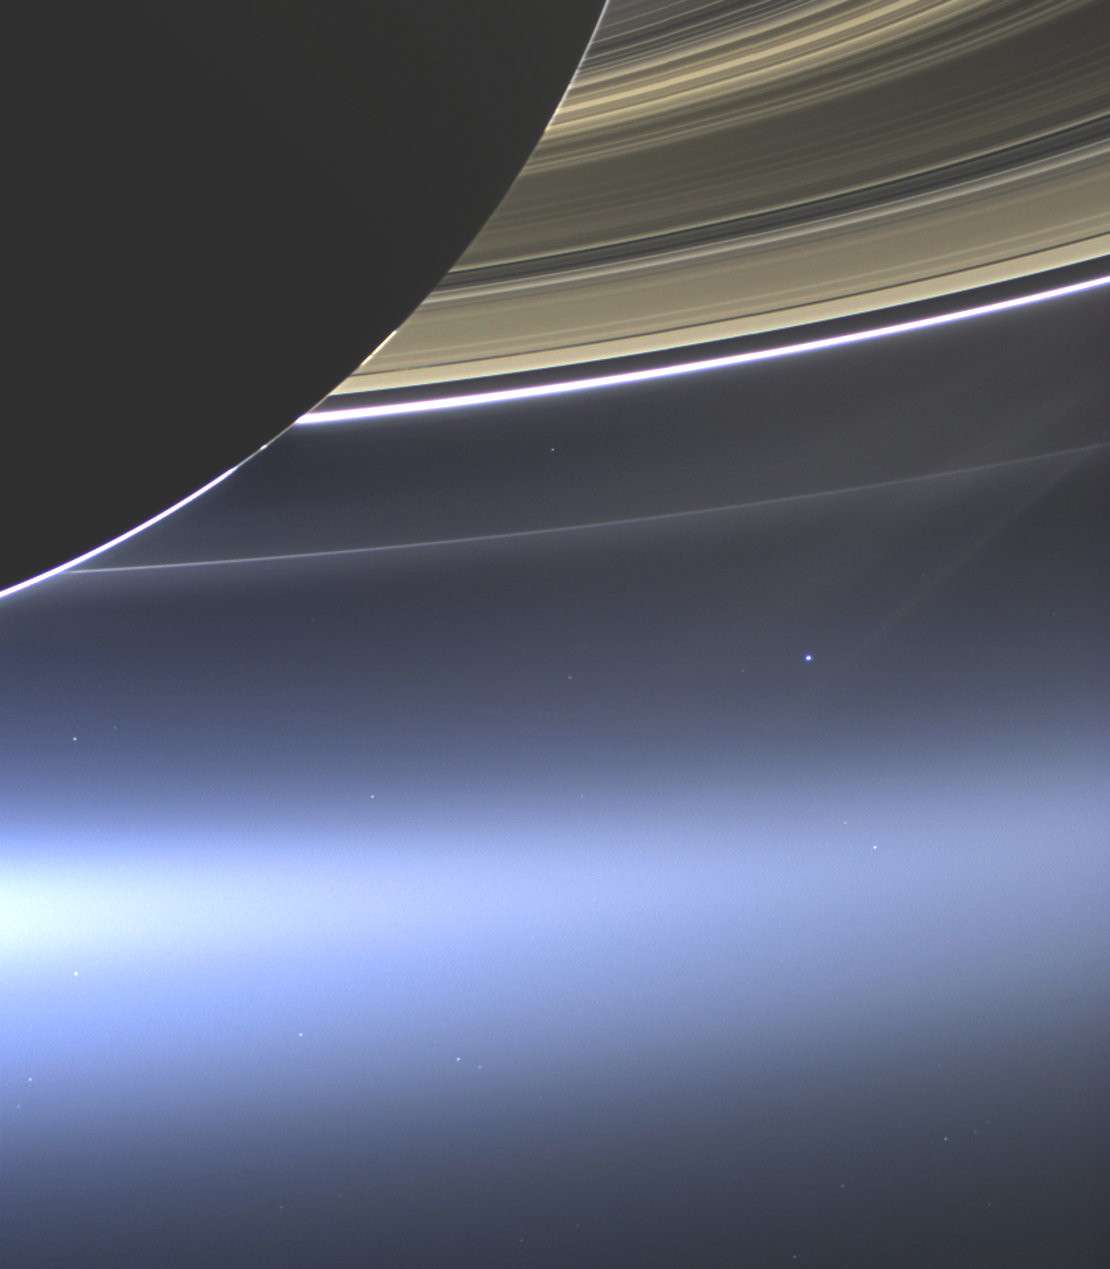
\includegraphics[width=0.5\textwidth]{Pale_Blue_Dot}
\end{wrapfigure}

Our posturings, our imagined self-importance, the delusion that we have some privileged position in the Universe, are challenged by this point of pale light. Our planet is a lonely speck in the great enveloping cosmic dark. In our obscurity, in all this vastness, there is no hint that help will come from elsewhere to save us from ourselves.

The Earth is the only world known so far to harbor life. There is nowhere else, at least in the near future, to which our species could migrate. Visit, yes. Settle, not yet. Like it or not, for the moment the Earth is where we make our stand.

It has been said that astronomy is a humbling and character-building experience. There is perhaps no better demonstration of the folly of human conceits than this distant image of our tiny world. To me, it underscores our responsibility to deal more kindly with one another, and to preserve and cherish the pale blue dot, the only home we've ever known.

